\documentclass[
    11pt,               % KOMA default
    a4paper,            % DIN A4
    %twoside,            % Zweiseitig
%     onside,
    headsepline,        % Linie unter der Kopfzeile
    %foodsepline,        % Linie �ber Fussnote
    %automark,           % Kolumnentitel lebendig
    %pointlessnumbers,   % Keinen Punkt hinter die letzte Zahl
                        % eines Kapitels (auch bei Anhang)
%     openleft,           %
    %openright,
    %cleardoubleplain,   %
    %abstracton,         %
    %idxtotoc,           % Index soll im Inhaltsverzeichnis auftauchen
    %liststotoc,         %
    %bibtotoc,           %
    %parskip            % parskip-, parskip*, parskip+
]%{scrreprt}
{scrartcl}

%\usepackage[latin1]{inputenc}
\usepackage[utf8]{inputenc}
\usepackage[ngerman]{babel}
\usepackage{graphicx}
\usepackage{subfigure}
\usepackage{float}
\usepackage{listings}
\usepackage{color}
\usepackage{tabularx}
\usepackage[hidelinks]{hyperref}
\usepackage{tabu}
\usepackage{booktabs}
\usepackage[table]{xcolor}
\usepackage{url}
\usepackage{lmodern}
\usepackage{amsmath}
\usepackage{amsfonts}
\usepackage{amssymb}
\usepackage{pdflscape}

\definecolor{dkgreen}{rgb}{0,0.6,0}
\definecolor{gray}{rgb}{0.5,0.5,0.5}
\definecolor{mauve}{rgb}{0.58,0,0.82}

\lstdefinelanguage{JavaScript}{
  keywords={typeof, new, true, false, catch, function, return, null, catch, switch, var, if, in, while, do, else, case, break},
  keywordstyle=\color{blue}\bfseries,
  ndkeywords={class, export, boolean, throw, implements, import, this},
  ndkeywordstyle=\color{darkgray}\bfseries,
  identifierstyle=\color{black},
  sensitive=false,
  comment=[l]{//},
  morecomment=[s]{/*}{*/},
  commentstyle=\color{purple}\ttfamily,
  stringstyle=\color{red}\ttfamily,
  morestring=[b]',
  morestring=[b]"
}

\lstset{
   language=JavaScript,
   backgroundcolor=\color{lightgray},
   extendedchars=true,
   basicstyle=\footnotesize\ttfamily,
   showstringspaces=false,
   showspaces=false,
   numbers=left,
   numberstyle=\footnotesize,
   numbersep=9pt,
   tabsize=2,
   breaklines=true,
   showtabs=false,
   captionpos=b
}

% Definitions
\definecolor{mydarkblue}{rgb}{0.0,0.0,0.5}
\definecolor{mylightblue}{rgb}{0.85,0.85,0.85}
\definecolor{mylightgray}{rgb}{0.95,0.95,0.95}

\newcommand{\HRule}{\rule{\linewidth}{0.4mm}}

\clubpenalty=10000
\widowpenalty=10000

\begin{document}

%\newpage
\pagestyle{empty}
\begin{center}
	
\includegraphics[scale=0.8]{images/hszg_logo.png}\\
	\vspace*{2cm}
	%\Large
	%\textbf{Fakultät}\\
	%\textbf{Elektrotechnik und Informatik}\\
	%\vspace*{2cm}
	\Huge
	\textbf{Belegarbeit}\\
	\Large
	\vspace*{2cm}
	\textbf{Ambient Assisted Living-Monitoringsystem mit eXist}\\
	\vspace*{5cm}
	
	\normalsize
	\newcolumntype{x}[1]{>{\raggedleft\arraybackslash\hspace{0pt}}p{#1}}
	\begin{tabular}{x{6cm}p{7.5cm}}
		\rule{0mm}{5ex}Kucera, Adam & {Matr.-Nr.:} 202549\\
		\rule{0mm}{5ex}Krause, Andre & {Matr.-Nr.:} 46932\\
		\rule{0mm}{5ex}Riedel, Robert & {Matr.-Nr.:} 202349\\

		\rule{0mm}{5ex}\textbf{Abgabedatum:} & \today \\ 
	\end{tabular} 
\end{center}
%\include{abstract}
\pdfbookmark{\contentsname}{toc}\tableofcontents
\thispagestyle{empty}

\newpage
\pagestyle{empty}
\listoffigures

%\newpage
%\listoftables

\newpage
\pagestyle{plain}
\setcounter{section}{0}
\pagenumbering{arabic}

\section{Einleitung}
\label{sec:Einleitung}
Der zunehmende Anteil der älteren Menschen in Staaten mit hoch entwickelter Industrie, wozu auch unter anderem Deutschland gehört, stellt in dem Sinne ein Problem dar, als dass eine Betreuung, falls benötigt, in den eigenen vier Wänden sich als sehr aufwändig gestaltet. Pflegeunternehmen kosten viel Geld und die eigene Familie ist nicht immer in der Lage, rund um die Uhr für die betroffene Person da zu sein. Da jedoch das Unabhängigkeitsgefühl und das gewohnte Zuhause eine große Rolle spielen, müssen andere Wege gefunden werden, um den Menschen ein altersgerechtes Wohnen bis in die späten Lebensjahre zu ermöglichen.
\\
\\
Hierfür gibt es bereits seit 2008 diverse Studien, die sich mit der Unterstützung durch technische Hilfsmittel beschäftigen. Das sogenannte \glqq Ambient-Assisted-Living\grqq \cite{aal} konzentriert sich dabei auf die Vernetzung des Wohnraumes an sich und mit externen Dienstleistern, um einerseits das alltägliche Leben durch spezielle Haushaltsgeräte oder Sicherheitssysteme zu unterstützen. Andererseits kann durch die Überwachung der vitalen Lebensfunktionen durch einen externen Dienstleister garantiert werden, dass im Notfall schnell Hilfe vor Ort ist \cite{aaltm}. Diese Überwachung kann beispielsweise durch am oder im Körper platzierte Sensoren, die die Vitalwerte messen und an eine Basisstation schicken, umgesetzt werden. Gleichzeitig werden diese Daten an eine zentrale Stelle, beispielsweise das Krankenhaus oder ein externer Dienstleister, gesendet, gespeichert sowie ausgewertet. Im Idealfall schränken solche Systeme den Nutzer in seinen alltäglichen Handlungen nicht ein und integrieren sich problemlos in sein Umfeld.

\begin{figure}[h]
\begin{center}
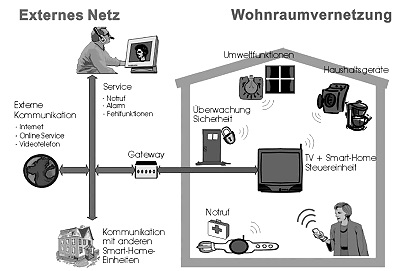
\includegraphics[scale=0.9]{images/intelligente-vernetzung.jpg} 
\caption{Schematische Darstellung eines AAL-Systems}
\end{center}
\end{figure}

\subsection{Problemstellung}
\label{subsec:Problemstellung}
In dem Projekt, was die folgende Arbeit näher beschreibt, sollte ein solches AAL-System zur Überwachung der vitalen Lebensfunktionen als eine Client-Server-Anwendung mit Hilfe von XML-Technologien umgesetzt werden. Dabei wird angenommen, dass es Sensoren gibt, die in regelmäßigen Abständen Vitalwerte an eine zentrale Einheit schicken. Diese Werte umfassen die Körpertemperatur, den Herzschlag, die Atemfrequenz sowie den Blutdruck. Die Werte werden in einer zentralen Datenbank mittels dem NoSQL-DBMS eXist abgespeichert, um zu jederzeit verschiedene Analysen über die gesammelten Werte erstellen zu können. Außerdem werden die Daten an eine Webapplikation geschickt, mit der sich alle Werte für eine bestimmte Person überwachen lassen. Sollte ein Wert eine kritische Grenze überschreiten, wird dem Nutzer eine visuelle sowie akustische Meldung ausgegeben, worauf dieser entsprechende Maßnahmen einleiten kann.

\newpage
\subsection{Aufgabenverteilung}
\label{subsec:Aufgabenverteilung}
Die Aufgaben im Team wurden folgendermaßen verteilt:

\begin{table}[H]
	\sffamily
	\caption{Aufgabenverteilung}
	\tabulinesep = 1mm %bringt die Reihen etwas weiter auseinander, angenehmer zu lesen
	\centering
		\begin{tabu} to 0.9\textwidth { X[1.7]  X[3] X[3]}
		\hline
		\textbf{Name} & \textbf{Programmierung} & \textbf{Belegteil}\\
		\hline 
		Kucera, Adam & \begin{itemize}
		\itemsep 0pt
		\item highCriticalValues.js
		\item index.html
		\item lowCriticalValues.js
		\item normalValues.js
		\item util.js
\end{itemize}		 & \begin{itemize}
		\itemsep 0pt
		\item 2.2.3. XSLT
		\item 2.2.4. Websockets
		\item 3.3 Vitalwerte Datengenerator
\end{itemize}\\ \hline
		Krause, Andre & \begin{itemize}
		\itemsep 0pt
		\item router.js
		\item index.js
		\item server.js
		\item socketServer.js
		\item vitalWerteHandler.js
		\item createReport.xqm
		\item getPersonId.xqm
		\item postSensorData.xqm
		\item test-xsl.xsl
\end{itemize} & \begin{itemize}
		\itemsep 0pt
		\item 1. Einleitung
		\item 1.1 Problemstellung
		\item 2.2.1 Node.JS
		\item 2.2.2. eXist
		\item 2.3 Systemarchitektur
		\item 2.4 Kommunikation (mit Robert Riedel)
		\item 3.1 Node.JS-Server
		\item 3.2 eXist-Server
		\item 4.1 Probleme
		\item A.2. Bedienungsanleitung
\end{itemize}\\ \hline
		Riedel, Robert & \begin{itemize}
		\itemsep 0pt
		\item clientFuntions.js
		\item clientPage.xhtml
		\item clientPageStyle.css
\end{itemize} & \begin{itemize}
		\itemsep 0pt
		\item \ref{subsec:UseCases} Use Cases
		\item \ref{subsec:Kommunikation} Kommunikation (mit Andre Krause)
		\item \ref{sec:Fazit} Fazit
		\item \ref{subsec:Ausblick} Ausblick
\end{itemize}\\
	\end{tabu}
\end{table}

\section{Entwurf}
\label{sec:Entwurf}
Im folgenden Kapitel wird der Entwurf der Anwendung näher beschrieben. Neben den Use Cases und den verwendeten Technologien, wird auch ein Überblick über die System-Architektur gegeben sowie die Kommunikation innerhalb des Systems näher erläutert.

\subsection{Use Cases}
\label{subsec:UseCases}
\begin{figure}[h]
\begin{center}
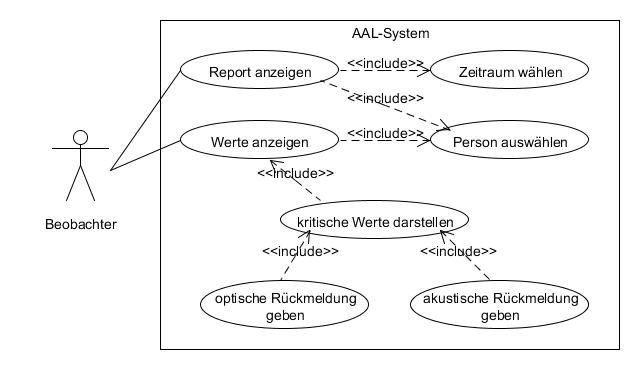
\includegraphics[scale=0.7]{images/AAL-Use-Case-Diagramm.jpg} 
\caption{Use Case Diagramm}
\label{fig:UseCaseDiagramm}
\end{center}
\end{figure}

Aus der Aufgabenstellung ergibt sich eine Reihe von Use Cases, welche in Abbildung~\ref{fig:UseCaseDiagramm} dargestellt sind. Der einzige Stakeholder ist ein \textit{Beobachter}. \textit{Beobachter} sind Personen, die die Werte einer Person, zu der Sensorwerte vorliegen, beobachtet. Beispiele für Beobachter sind z.B. Pfleger oder Angehörige. In erste Linie möchte ein \textit{Beobachter}, das die zu der Beobachteten Person passenden Werte angezeigt werden(Use Case:\textit{Werte anzeigen}). Dazu ist es nötig, dass diese Person zuerst ausgewählt wird(Use Case:\textit{Person auswählen}). Um die Werte sinnvoll darzustellen, müssen vor allem kritische Werte gesondert dargestellt werden, da diese meist eine Bedrohung für Leib und Leben der beobachten Person darstellen. Zu diesem Zweck gibt es zum einen eine optische Rückmeldung(Use Case:\textit{optische Rückmeldung geben}) und zum anderen eine akustische(Use Case:\textit{akustische Rückmeldung geben}).\\
Neben der zeitnahen Überwachung der Werte soll es ebenfalls möglich sein eine Zusammenstellung vergangener Werte zu erhalten(Use Case:\textit{Report anzeigen}). Auch dazu muss zuvor die gewünschte Person ausgewählt werden, aber zusätzlich auch ein Datumszeitraum(Use Case:\textit{Zeitraum wählen}).\\
Werden die in diesen Use Cases definierten Grundanforderungen erfüllt, entsteht eine einfache Applikation zur Überwachung von Sensorwerten.


\subsection{Technologien}
\label{subsec:Technologien}
Die folgenden Technologien wurden im Projekt eingesetzt und sollen für das Verständnis näher erläutert werden.

\subsubsection{Node.JS}
\label{subsec:NodeJS}
Node.JS \cite{nodejswebsite} bringt die Programmiersprache Javascript auf die Server-Ebene. Üblicherweise werden Sprachen wie PHP zur Erstellung von Webservices genutzt, um Anwendungen durch Anfragen eines Clients zu starten. Diese Architektur ist jedoch in solchen Fällen ungeeignet, in denen der Client in Echtzeit über Änderungen informiert werden soll. Node.JS ermöglicht es nun Webservices zu erstellen, die mittels Javascript von Anfragen der Clients unabhängig ausgeführt werden können. Hierzu wird die Anwendung beim Start an einen TCP-Port gebunden und erwartet die Anfragen vom Client. Im folgenden Codebeispiel \ref{lst:hellonode} ist gut zu erkennen, dass mit wenig Aufwand ein \textit{"Hello World"}-Server erstellt werden kann.

\begin{lstlisting}
var http = require('http');
http.createServer(function (req, res) {
  res.writeHead(200, {'Content-Type': 'text/plain'});
  res.end('Hello World\n');
}).listen(1337, '127.0.0.1');
console.log('Server running at http://127.0.0.1:1337/');
\end{lstlisting}

Außerdem kann nun aktiv mit dem Client über die geöffnete Verbindung kommuniziert werden. Zum Einsatz kommt dabei die Javascript Engine V8, welche auch im Google Chrome Browser eingesetzt wird. Die besonderen Eigenschaften von Node.JS liegen darin, schnelle und ressourcensparende Webservices zu ermöglichen, die außerdem viele gleichzeitige Anfragen von Clients bewältigen können \cite{cantelon:nodejs}. Dies wird zum einen durch die Auslagerung des I/O-Systems, also den Lese- und Schreiboperationen, in externe Prozesse realisiert. Dadurch werden Abläufe nicht durch die I/O-Operationen blockiert, sondern asynchron verarbeitet. Singlethreading ermöglicht außerdem das Vermeiden von parallelen Zugriffen auf bestimmte Ressourcen, so wie es bei Multithreading der Fall ist. Es müssen sich also keine Gedanken um eventuelle Thread-Safety-Implementierungen gemacht werden. Node.JS bietet ein reichhaltiges Angebot an Zusatzpaketen, die die bestehenden Funktionen erweitern. So ist es möglich z.B. REST-Services oder das Parsen von XML-Dokumenten leicht zu implementieren. Der im Node.JS enthaltene Package Manager (\textit{npm}) lädt alle nötigen Bibliotheken und stellt sie zur Verfügung.

\subsubsection{eXist}
\label{subsec:eXist}
eXist \cite{existwebsite} ist eine in der Sprache Java entwickelte Anwendung, die in ihrer Ursprungsform als eine native XML Datenbank gedacht war \cite{siegel:exist}. Mittlerweile befindet sich das Projekt in der Version 2.2 und umfasst zahlreiche Funktionen, die es ermöglichen, XML-basierte Anwendungen zu erstellen sowie Dokumente in einer NoSQL-Datenbank abzuspeichern und zu verwalten. Die Abfragesprache XQuery\footnote[1]{XML Query Language} ermöglicht das Zugreifen auf die gespeicherten Dokumente. Es können jedoch nicht nur XML-Dokumente in der Datenbank abgelegt werden, sondern nahezu jedes Dateiformat ist erlaubt. So lassen sich eben auch Anwendungen erstellen, die andere Technologien verwenden.
\\
\\
In der stetigen Entwicklung von eXist kam auch eine grafische Oberfläche hinzu, mit der z.B. Code direkt über eine integrierte IDE erstellt und verändert werden kann. Eine Erweiterung des Funktionsumfangs ist durch den Paketmanager leicht möglich. eXist befindet sich weiterhin in der Entwicklung und manche Funktionen sind noch nicht fertig implementiert oder haben noch Fehler. Es ist jedoch in dem jetzigen Stand sehr gut nutzbar.

\subsection{Systemarchitketur}
\label{subsec:Systemarchitketur}
Bei der Systemarchitektur fiel die Wahl auf eine Client-Server Anwendung. Aufgrund der Anforderung, ein Monitoring-System zu erstellen, sprich das der Nutzer über eine grafische Schnittstelle bestimmte Werte angezeigt bekommen lassen möchte, musste ein Client erstellt werden. Weiterhin war gefordert, dass Sensoren von verschiedenen Haushalten aus Daten an das Monitoring-System schicken und diese auch gespeichert werden. Daher musste es eine Möglichkeit geben, die Daten von verschiedenen Quellen in einer zentralen Einheit verwalten zu können. Hierfür wurde ein Server mit integrierter Datenbank ausgewählt. Der erste Entwurf für die Systemarchitektur sah wie folgt aus:

\begin{figure}[h]
\begin{center}
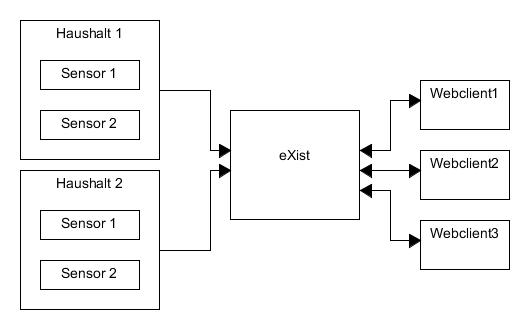
\includegraphics[scale=0.6]{images/sa1.jpg} 
\caption{Erster Entwurf Systemarchitektur}
\end{center}
\end{figure}

Ein eXist-Server stellt dabei die zentrale Komponente dar, die sowohl alle Daten von den Sensoren entgegennimmt und verwaltet, sowie auch für die Kommunikation zwischen dem Server und den Clients verantwortlich ist. Für die Sensoren stellt der Server einen REST-Service zur Verfügung, welcher als Übertragungsschnittstelle der ermittelten Vitalwerte dient. So ist es auch leicht möglich, weitere Sensoren an das System anzuschließen, da lediglich die Adresse des REST-Services bekannt sein muss und in welcher Form die Daten übertragen werden müssen. Ansonsten gibt es keine direkte Kopplung. Für die Kommunikation zwischen Server und Clients hätte ebenfalls ein REST-Service verwendet werden können. Hierbei hätte sich jedoch das Problem ergeben, dass sich die Daten von den Sensoren in sehr kurzen Zeitabständen ändern. Um jedoch immer die aktuellsten Vitalwerte anzeigen zu können, müsste der Client sehr oft den Server nach neuen Daten abfragen. Bei mehreren Clients könnte dies zu einer Serverüberlastung führen, da der Server nicht mehr alle Anfragen in kurzer Zeit beantworten kann.
\\
\\
Daher wurde entschieden, die Kommunikation mittels Websockets zu realisieren. Der Vorteil besteht darin, dass der Client nur einmal die Verbindung zum Server aufbaut und dieser dann die Verbindung nutzt, um Daten an den Client zu schicken, ohne dass dieser sich neu verbinden muss. Dies eignet sich besonders gut für das Monitoring-System: Sobald die Sensoren neue Daten schicken, können diese direkt an den wartenden Client weitergeleitet werden, der bereits die Verbindung geöffnet hat und in dem Sinne empfangsbereit für jede Änderung ist. Mit eXist ist eine solche Kommunikationsart nicht möglich, da es keine solche Implementierung der Websockets besitzt. Aus diesem Grund wurde ein zweiter Server hinzugenommen, der sowohl eine REST-Schnittstelle, als auch Websockets zur Verfügung stellt. Die Wahl fiel dabei auf einen Node.JS-Server, da dieser sehr ressourcensparend ist und viele gleichzeitige Netzwerkverbindungen ermöglicht. Der neue Entwurf für die Systemarchitektur ist nun wie folgt:

\begin{figure}[h]
\begin{center}
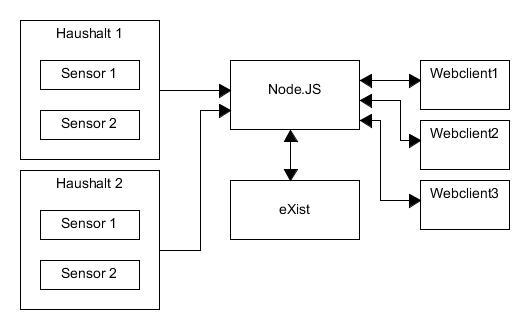
\includegraphics[scale=0.6]{images/sa2.jpg} 
\caption{Zweiter Entwurf Systemarchitektur}
\end{center}
\end{figure}

Der Node.JS-Server ist die zentrale Einheit und steuert die Kommunikation zwischen den Sensoren und den Clients. Weiterhin speichert er alle empfangenen Werte in der eXist-Datenbank ab. Hauptsächlich besteht die Aufgabe des Node.JS-Servers darin, die Anfragen und Antworten an die entsprechenden Stellen (eXist, Client) weiterzuleiten. Dies war jedoch nötig, um sowohl REST-Services, als auch Websockets verwenden zu können.

\subsection{Kommunikation}
\label{subsec:Kommunikation}
Die Sensoren schicken ihre ermittelten Werte (\textit{sensorData}) an den Node.JS -Server. Dabei wird die Antwort von den Sensoren jedoch ignoriert, da auf dieser Seite keine  Fehlerbearbeitung vorgesehen ist. Die Daten werden über eine REST-Anfrage (POST) mit dem entsprechenden XML-Dokument gesendet.

\begin{figure}[h]
\begin{center}
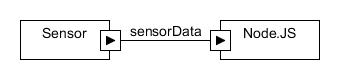
\includegraphics[scale=0.6]{images/komm1.jpg} 
\caption{Kommunikation zwischen Sensoren und Node.JS-Server}
\end{center}
\end{figure}

Der eXist-Server bietet zur Kommunikation einen Standard, mit dem sich mittels XQuery REST-Services erstellen lassen. \textit{RESTXQ} bietet verschiedene Annotationen, um beispielsweise einen URL-Pfad anzugeben, unter dem eine Funktion von außerhalb angesprochen werden kann, oder um die Funktion als eine POST-Methode festzulegen. Mit Hilfe der Annotationen wurde nun die Kommunikation zwischen dem Node.JS-Server und der eXist-Datenbank hergestellt. Die von den Sensoren empfangenen Daten werden mittels POST an die Datenbank geschickt (\textit{sensorData}). Weiterhin kann mittels einem \textit{reportRequest} ein Report für eine bestimmte Person in einem Zeitraum über alle Vitalwerte angefordert werden. Der eXist sendet daraufhin die erstellte PDF-Datei als \textit{reportData} wieder zum Node.JS-Server. Außerdem kann geprüft werden, ob eine \textit{personId} in der Datenbank bereits verzeichnet ist. Dafür sendet der Node.JS-Server eine Anfrage mit der \textit{personId} an eXist und erhält eine Meldung über die Existenz der ID (\textit{personIdResponse}).

\begin{figure}[h]
\begin{center}
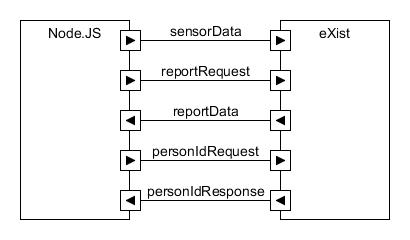
\includegraphics[scale=0.6]{images/komm2.jpg} 
\caption{Kommunikation zwischen Node.JS-Server und eXist}
\end{center}
\end{figure}

Von den Clients aus können sowohl die Reports, als auch die Überprüfung der gewünschten \textit{personId} angefordert werden. Der Node.JS-Server leitet diese Anfragen an eXist weiter und gibt die Antworten an die Clients zurück. Diese Anfragen hätten auch über einen REST-Service erstellt werden können, man entschied sich aber dafür, die Kommunikationsarten auf Clientseite nicht zu vermischen. Außerdem erhält der Client über die offene Websocket-Verbindung jeden neuen Wert, der von den Sensoren geschickt wurde.  \\ \\

\begin{figure}[h]
\begin{center}
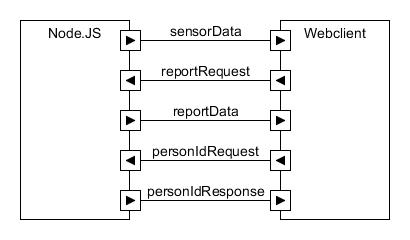
\includegraphics[scale=0.6]{images/komm3.jpg} 
\caption{Kommunikation zwischen Node.JS-Server und Client}
\end{center}
\end{figure}

Zur Übermittlung der Daten von den Sensoren zum Server wurde eine XML-Struktur verwendet, welche in Abbildung~\ref{lst:sensorXml} zu sehen ist.
Die \texttt{personId} identifiziert die Person, der der gesendete Datensatz zugeordnet wird. Die \texttt{roomId} symbolisiert den Aufenthaltsort der Person, wobei der Wert auch eine Abstrakte Id sein kann und keine physische Lokalität. Der \texttt{timestamp} beinhaltet die Uhrzeit und das Datum der Erfassung des Datensatzes. Das gewählte Format richtet sich dabei nach der Speicherung im eXist um die Verarbeitung dort zu erleichtern. Der \texttt{sensor} Tag beinhaltet den Typ (\texttt{type}) des Sensors und seinen Wert(\texttt{value}). Durch die separate Angabe des Typs als Textwert in der XML ist es leicht möglich diese XML-Struktur für weitere Sensortypen zu verwenden. Ebenso kann der Wert sehr allgemein geschickt werden, z.B. auch als String mit physikalischer Einheit. Der \texttt{status} kann genutzt werden um direkt zu übermitteln, ob ein Wert in einem kritischen Bereich liegt. Dadurch ist es nicht nötig, dass der Empfänger Kenntnis von den Grenzwerten hat.

\begin{lstlisting}[caption={SensorXML},label=lst:sensorXml]
<sensorData>
   <personId>Andre</personId>
   <roomId>Wohnzimmer</roomId>
   <timestamp>
      <time>15:33:58 PM</time>
      <date>2015-06-24</date>
   </timestamp>
   <sensor>
      <type>Herzschlag</type>
      <value>120</value>
   </sensor>
</sensorData>
\end{lstlisting}

\section{Implementierung}
\label{sec:Implementierung}
Das folgende Kapitel beschreibt beispielhaft die Umsetzung des im vorigen Abschnitt beschriebenen Entwurfs. Dabei wird auf einzelne Programmabschnitte näher eingegangen.

\subsection{Node.JS-Server}
\label{subsec:NodeJSServer}
Der Node.JS-Server besteht aus zwei Instanzen. Eine Instanz ist als ein REST-Service implementiert. Sie stellt eine POST-Ressource zur Verfügung, über die die Daten der Sensoren an das eXist geschickt werden. Hierfür gibt es eine \textit{route}-Funktion, die ein Request entgegennimmt und prüft, welche URL angesprochen wird. 

\begin{lstlisting}
function route(handle, pathname, response, request) {
    if(typeof handle[pathname] === 'function'){
        handle[pathname](response, request);
    } else {
        console.log("No request handler found for " + pathname);
        response.writeHead(404, {"Content-Type": "text/plain"});
        response.write("404 Not found");
        response.end();
    }
}
\end{lstlisting}

Node.JS extrahiert den \textit{pathname}, also den Teil der URL, der nach dem Host und der Portnummer folgt, automatisch. Sollte die URL nicht zu einer Funktion zuzuordnen sein, wird ein 404-Fehler zurückgegeben mit dem Hinweis, dass die Ressource nicht gefunden wurde.

\begin{lstlisting}
handle["/postVitalwert"] = vitalWerteHandler.postVitalwert;
\end{lstlisting}

Wenn aber die URL wie im obigen Beispiel \textit{postVitalwert} ist, wird die entsprechende Funktion \textit{postVitalwert} ausgeführt. Diese Funktion sendet die empfangenen Daten an eXist weiter. Um REST-Calls in Node.JS durchzuführen, wurde das Package \textit{node-rest-client} zusätzlich installiert. Ein POST kann wie folgt implementiert werden.

\begin{lstlisting}
client.post("http://localhost:8080/exist/restxq/postSensorData", args, function(data,response) {
    var string = data.message;
});
\end{lstlisting}

Dadurch wird ein POST an die angegebene Adresse mit den spezifischen Daten in \textit{args} ausgeführt. Die Antwort wird in der übergebenen Callback-Funktion verarbeitet. Außerdem  werden die Daten von den Sensoren an die zweite Instanz des Node.JS-Servers weitergeleitet.
\\
\\
Die zweite Instanz ist für die Kommunikation zwischen den Clients und dem Server verantwortlich. Diese wird durch den Einsatz von Websockets realisiert. Das Package \textit{socket.io} ermöglicht das Erzeugen einer Connection sowie das Senden und Empfangen von Events. Sobald sich ein Client über den Socket angemeldet hat, kann auf solche Events reagiert werden.

\begin{lstlisting}
socket.on("setPersonId", function(id){
            ...
});
\end{lstlisting}

In diesem Beispiel wird beim empfangenen Event \textit{setPersonId} die Callback-Funktion mit der empfangenen ID ausgeführt. Es können aber auch Events an die angemeldeten Clients mittels der Funktion \textit{emit} geschickt werden.

\begin{lstlisting}
receiver.emit("receiveVitalWert", xml);
\end{lstlisting}

Die beiden Instanzen wurden jeweils an zwei verschiedene Ports gebunden, um z.B. zu vermeiden, dass ein Websocket-Event an den Router des REST-Services geschickt wird. Deshalb wurde für den REST-Service der Port 8888 und für den Websocket-Service der Port 8887 festgelegt.

\subsection{eXist-Server}
\label{subsec:eXistServer}
Um eXist von außerhalb ansprechen zu können, wurde der in eXist implementierte Standard \textit{RESTXQ} verwendet. Dieser ermöglicht mittels Annotationen das Bereitstellen von \textit{resource functions}, also Ressourcen, die über HTTP verfügbar sind. Es können XQuery-Funktionen über solche HTTP-Anfragen ausgeführt und die Ergebnisse zurückgegeben werden. POST-Methoden werden beispielsweise mit der Annotation \textit{\%rest:POST("\{\$body\}")} deklariert. Mit dem \textit{\$body} Element kann außerdem festgelegt werden, dass mit dem POST Daten gesendet werden sollen.

\begin{lstlisting}
declare
    %rest:POST("{$body}")
    %rest:consumes("application/xml")
    %rest:path("/postSensorData")
function ex:postSensorData($body){
    ...
};
\end{lstlisting}

Außerdem ist es möglich, eine Antwort an den anfragenden Client innerhalb von XQuery zu erstellen. Das Element \textit{$<$rest:response$>$} erzeugt mit dem Kindelement \textit{$<$http:response$>$} eine HTTP Statusmeldung mit optional angehangenen Daten. Im folgenden Beispiel wird nach erfolgreichem Speichern der Vitalwerte ein Statuscode 200 gesendet mit dem kurzen XML-Dokument \textit{$<$message$>$Document updated$<$/message$>$}

\begin{lstlisting}
<rest:response>
     <http:response status="200" message="ok">
     <http:header name="Content-Type" value="application/xml"/>
     <http:header name="Access-Control-Allow-Origin" value="*"/>
</http:response>
</rest:response>,<message>Document updated</message>
\end{lstlisting}

Für die Erstellung der Reports wurde XSLT\footnote[1]{XSL Transformation} und XSL-FO\footnote[2]{Extensible Stylesheet Language – Formatting Objects} verwendet. 

\begin{lstlisting}
let $table-fo := transform:transform($tableBody,doc("/db/apps/aal-server/test-xsl.xsl"),())
let $fo := <fo:root xmlns:fo="http://www.w3.org/1999/XSL/Format">
    <fo:layout-master-set>
        <fo:simple-page-master master-name="my-page">
            <fo:region-body margin="1in"/>
        </fo:simple-page-master>
    </fo:layout-master-set>
    <fo:page-sequence master-reference="my-page">
        <fo:flow flow-name="xsl-region-body">
            <fo:block>
                {$table-fo}
            </fo:block>
        </fo:flow>
    </fo:page-sequence>
</fo:root>
let $pdf := xslfo:render($fo, "application/pdf", ())
\end{lstlisting}

In der ersten Zeile wird das XML-Dokument, welches transformiert werden soll sowie die XSL-Datei, die alle Regeln zur Transformation enthält, mittels der Funktion \textit{transform:transform} umgewandelt. In diesem Fall entsteht eine Tabelle mit allen wichtigen Daten. eXist benutzt als XSLT-Prozessor standardmäßig \textit{Saxon HE}. Danach wird in den Zeilen 2 bis 15 ein XSL-FO-Dokument erstellt, welches Layout-Optionen für die PDF beinhaltet. Außerdem wird die transformierte XML als der Körper der PDF im Element \textit{$<$fo:block$>$} deklariert. In Zeile 16 entsteht durch die Funktion \textit{xslfo:render} das fertige PDF-Dokument. Dies kann nun an den Client als ein Base64 codierter String zurückgegeben und im Browser angezeigt werden. \textit{Apache FOP} ist in eXist der standardmäßige Renderer, der genutzt wird um die XSL-FO-Dokumente zu rendern. 
\\
\\
Da eXist aus einem NoSQL-DBMS besteht, werden alle Daten in Dokumenten abgespeichert. Dazu enthält die in diesem Projekt erstellte Datenbank für jede Person eine Collection (Siehe Abbildung \ref{collection1} auf S. \pageref{collection1}) mit der entsprechenden personId als Namen, um für die Reports gezielt nur die Dokumente zu durchsuchen, die notwendig sind. Innerhalb der Collections werden für jeden Tag separate XML-Dokumente (Siehe Abbildung \ref{collection2} auf S. \pageref{collection2}) erstellt, die alle Vitalwerte für die jeweilige Person enthalten.
\subsection{Vitalwerte Datengenerator}
Am Anfang war es wichtig, die vitale Werte d.H. Atemfrequenz, Herzfrequenz, Körpertemperatur und Blutdruck erzeugen lassen. Für die Darstellung kommt eine HTML Webseite mit Javascript und Jquery Technologien vor.

Um diese Aufgabe zu erreichen, wurde erst einfacher Formular erstellt.
Dieser besteht aus drei wichtigen Eingabefeldern, sprich Person ID, Room ID und Change room. Damit kann man eine fiktive Person mit einen Namen und einer Position darstellen. Um eine Bewegung zu simulieren, ist es später möglich das Zimmer zu ändern. Zusätzlich gibt es noch ein Start-und Stop Knopf für Ein-und Auschaltung des Generators.
 
Nachdem Einschalten werden die Werte für Atemfrequenz und Herzfrequenz jede 5 und für die Körpertemperatur und Blutdruck jede 10 Sekunden generiert. Die Werte werden inzwischen dem normalen Intervall erzeugt. Normaler Intervall enstspricht dem gesunden Menschen. Um den besseren Verständnis über die ganze Situation zu bekommen, besteht den Nutzern eine Möglichkeit die generierten vital Werte live zu beobachten und auch steuern. Der Nutzer kann die Werte erhöhen oder vermindern.

Sollten die Werte außerhalb des normalen Intervalles liegen, kommt es zur Warnung mit dem akustischen Signal. 
Der zweiten Element der Webseite ist eine Tabelle, die die neu generierten Werte zeigt. Dort sieht man die neue Werte, jetzige Person ID, Room ID und auch entsprechenden Zeitstempel. Es gibt auch s.g. Normalspalte, wo man der normalen Intervall sehen und auch mit neuen Werten vergleichen kann.
\\
\begin{lstlisting}
function generateBodyTemp() {
//from 35.8 to 37.3 Celsius
var x = parseFloat(Math.random() * 1.5 + 35.8).toFixed(2);
document.getElementById("bodyTemp").innerHTML = x;

var personId = document.getElementById("personid").value;
var roomId = document.getElementById("pokojid").innerHTML;
var time = displayTime();
var date = getDate();
var sensorType = "Koerpertemperatur"; 
var string = xmlString(personId, roomId, time, date, sensorType, x);

ajax(string);    
}
\end{lstlisting}

Zum Erläuterung des Generatorhintegrundes wurde eine Funktion generateBodyTemp genommen, die die fiktive Körpertemperatur erzeugt. Die restlichen Vitalwerte Funktionen basieren auf das gleichem Prinzip. Unser Ziel ist die Herstellung von Nummer in dem Intervall von 35.8 bis 37.3. In der dritten Zeile geht es um die zufällige Erzeugung des Wertes. Mit der Methode getNumberFromInterval kann man mittels dieser Formula die zufälligen Nummer in dem beliebigen Intervall herstellen. 
\begin{lstlisting}
var getNumberFromInterval = Math.random() * (max - min) + min;
\end{lstlisting}

Dazu wurde die Methode Math.random benutzt, die eine Nummer zwischen 0 und 1 liefert. Danach wird die Nummer mit 1.5 multipliziert und dazu noch 35.8 addiert. Mit der parseFloat Methode nimmt man den String und liefert eine Fließkommazahl zurück.  Die Methode toFixed konvertiert die Nummer in den String mit 2 Stellen nach dem Dezimalkomma. Die neue Nummer wird in die Variable x gespeichert. In der vierten Zeile wird den neu generierten Wert in der HTML Tabelle mittels getElementById Methode gezeigt.

In den Zeilen 6 und 7 werden die von dem User eingegebene Werte in den Variablen gespeichert. Die Zeilen Nr. 8 und 9 sind für die Herstellung des Zeitstempels zuständig. Dazu sind 2 Funktionen vorhanden und die Werte werden auch in den Variablen gespeichert. Die Zeile Nr. 10 beinhaltet den String Körpertemperatur. In der 11. Zeile wird die Funktion xmlString mit dem Parameter 6 benutzt. Diese Methode erhält die Parameter und speichert sie in die Variable string.

In der letzten Zeile wird die Funktion ajax mit dem Parameter string aufgerufen.
\\
\begin{lstlisting}
function ajax(string){
$.ajax({
url: 'http://uakk45c08dae.aalxmlprojekt.koding.io:8888/postVitalwert', 
processData: false,
type: "POST",
data: string,
crossDomain: true,
success: function(response){
console.log("Success!");
},
error: function(jqXHR, textStatus, errorThrown) {
console.log(errorThrown + ", " + jqXHR);
}
});
}
\end{lstlisting}

Die oben genannte Funktion ajax dient zum Übertragung der Daten zum Server. In der dritten Zeile spezifiziert man, zu welcher Adresse sich ajax verbindet. Die Variable string wird via POST Methode zu der URL gesendet. ProcessData ist auf false gesetzt, weil man das DOMDocument senden möchte. CrossDomain ist auf true gesetzt um die crossDomain Anforderungen verwenden zu können. Wenn die Daten erfolgreich zum Server gesendet werden, taucht die console mit dem Wert Success auf. Wenn aus irgendwelchen Gründen die Übertragung nicht ausgeführt werden kann, liefert die Funktion einen Error zurück.   
     


%======================================================================
%   Literaturverzeichnis
%======================================================================
\renewcommand{\baselinestretch}{1.13}\normalsize
\markboth{BIBLIOGRAPHY}{BIBLIOGRAPHY}
\renewcommand{\bibname}{BIBLIOGRAPHY}
\bibliographystyle{plaindin}
\selectlanguage{ngerman}
\bibliography{literatur}
\cleardoublepage

%======================================================================
%   Selbstständigkeitserklärung
%======================================================================
\selectlanguage{ngerman}
\section*{Selbstständigkeitserklärung}
\thispagestyle{empty} Hiermit erkläre ich, dass ich die vorliegende
Arbeit selbstständig angefertigt, nicht anderweitig zu
Prüfungszwecken vorgelegt und keine anderen als die angegebenen
Hilfsmittel verwendet habe. Sämtliche wissentlich verwendete
Textausschnitte, Zitate oder Inhalte anderer Verfasser
wurden ausdrücklich als solche gekennzeichnet.%\\[2ex]

\vspace{2cm}\noindent
%--------------------------------- \newline
\vspace{1cm}\noindent
--------------------------------- \newline
\vspace{1cm}\noindent
--------------------------------- \newline
\vspace{1cm}\noindent
--------------------------------- \newline

Görlitz, \today

\end{document}